\textit{Response.} 

\begin{enumerate}[a)]
	\item To show that the switching times are given by Eqs.~\ref{eqs:switching_times}, we first consider the definition og the switching rates. In particular, the switching rate $\lambda_{i,j}$ from state $i$ to state $j$ is defined as
	
		\begin{equation}
			\lim_{\Delta t \to 0^{+}} \frac{\func{p_{\Delta t}}{i,\ j}}{\Delta t} = \lambda_{i,j}
		\end{equation}
		
		where $\func{p_{\Delta t}}{i,\ j}$ is the probability that the process goes from state $i$ to state $j$ in a time interval of length $\Delta t$. In other words, for this two-state Markov process we have
	
		\begin{subequations}
			\begin{align}
				\func{p_{\Delta t}}{s_{st},\ s_{un}} &= \nu\,\Delta t + \func{\text{o}}{\Delta t},\\
				\func{p_{\Delta t}}{s_{un},\ s_{st}} &= \mu\,\Delta t + \func{\text{o}}{\Delta t}.
			\end{align}
		\end{subequations}
		
		From these, we may obtain the probability that the state remains the same after a time interval of length $\Delta t$
		
		\begin{subequations}
			\begin{align}
				\func{p_{\Delta t}}{s_{st},\ s_{st}} &= 1 - \nu\,\Delta t + \func{\text{o}}{\Delta t},\\
				\func{p_{\Delta t}}{s_{un},\ s_{un}} &= 1 - \mu\,\Delta t + \func{\text{o}}{\Delta t}.
			\end{align}
		\end{subequations}
		
		Therefore, to find the probability that the time that the state remains in $s_{st}$ until a given time $t$, i.e., $\func{P}{T_{st} \leq t}$, we may discretize the interval $\gbkt{0,\ t}$ into $n$ sub-intervals of length $\Delta t$.\footnote{By time-homogeneity of the two-state Markov jump process, we may pick the interval $\gbkt{0,\ t}$, and our argument will apply to all time intervals of length $t$.} Writing $t = n\,\Delta t$, we have
		
		\begin{align}
			\func{P}{T_{st} \leq t} &= \func{p_{t}}{s_{st},\ s_{st}} \nonumber \\
				&\approx \func{p_{n\,\Delta t}}{s_{st},\ s_{st}} \nonumber \\
				&= \gpr{\func{p_{\Delta t}}{s_{st},\ s_{st}}}^n \nonumber \\
				&= \gpr{1 - \nu\,\Delta t + \func{\text{o}}{\Delta t}}^n \nonumber \\
				&= \gpr{1 - \frac{\nu\,t}{n} + \func{\text{o}}{\frac{t}{n}}}^n,
		\end{align}
		
		where the fourth equality follows from the third by the Markov property of the Markov jump process. The limit of $n \to \infty$ corresponds to an infinitely refined discretization of the interval $\gbkt{0,\ t}$, i.e.,
		
		\begin{align}
			\func{P}{T_{st} \leq t} &= \lim_{n \to \infty} \func{p_{t}}{s_{st},\ s_{st}} \nonumber \\
				&= \lim_{n \to \infty} \gpr{1 - \frac{\nu\,t}{n} + \func{\text{o}}{\frac{t}{n}}}^n \nonumber \\
				&= 1 - e^{-\nu t},
		\end{align}
		
		as desired. We may similarly obtain the desired equation for $\func{P}{T_{un} \leq t}$.
		
		Now, from the equilibrium distribution 
		
		\begin{subequations}
			\begin{align}
				\func{p_{eq}}{s,\ s_{un}} &= \frac{\nu}{\nu + \mu} = \func{p_{eq}}{s_{un}}, \\
				\func{p_{eq}}{s,\ s_{st}} &= \frac{\mu}{\nu + \mu} = \func{p_{eq}}{s_{st}}, \\
			\end{align}
		\end{subequations}
		
		where $s \in \mathcal{S}$, and the second equalities on the right follow from the independence of $\func{p_{eq}}{s,\ s_{un}}$ and $\func{p_{eq}}{s,\ s_{st}}$ on $s$. We may find the expected state after a long time
		
		\begin{equation}
			\ev{X} = s_{un}\,\func{p_{eq}}{s_{un}} + s_{st}\,\func{p_{eq}}{s_{st}} = \frac{\nu\,s_{un} + \mu\,s_{st}}{\nu + \mu}.
		\end{equation}
		
	\item Source code is available from the GitHub repository
	
\begin{center}
	\url{https://github.com/jasonltorchinsky/MATH833_HW/releases/tag/hw2}
\end{center}

and is given in Appendix~\ref{app:code_2}. In short, the code takes a input parameters \texttt{-{}-n} (or \texttt{-N}), that corresponds to the number of transitions we wish to simulate. To simulate the two-state Markov jump process, we generate a discrete-time Markov chain $Y_n$ and a sequence $\gbrc{\Delta t_i}_{i = 0}^{n-1}$ of exponentially distributed transition times based on $Y_n$. For example, if $Y_4 = s_{st}$, then $\Delta t_4$ is an exponentially distributed random variable with decay parameter $\nu$. The continuous-time Markov chain $X_t$ is then simply $Y_j$ at time $\sum_{i = 0}^{j} \Delta t_i \leq t \leq \sum_{i = 0}^{j+1} \Delta t_i$. We give a sample trajectory including 20 trajectories in Figure~\ref{fig:traj_2}.

\begin{figure}[H]
	\centering
	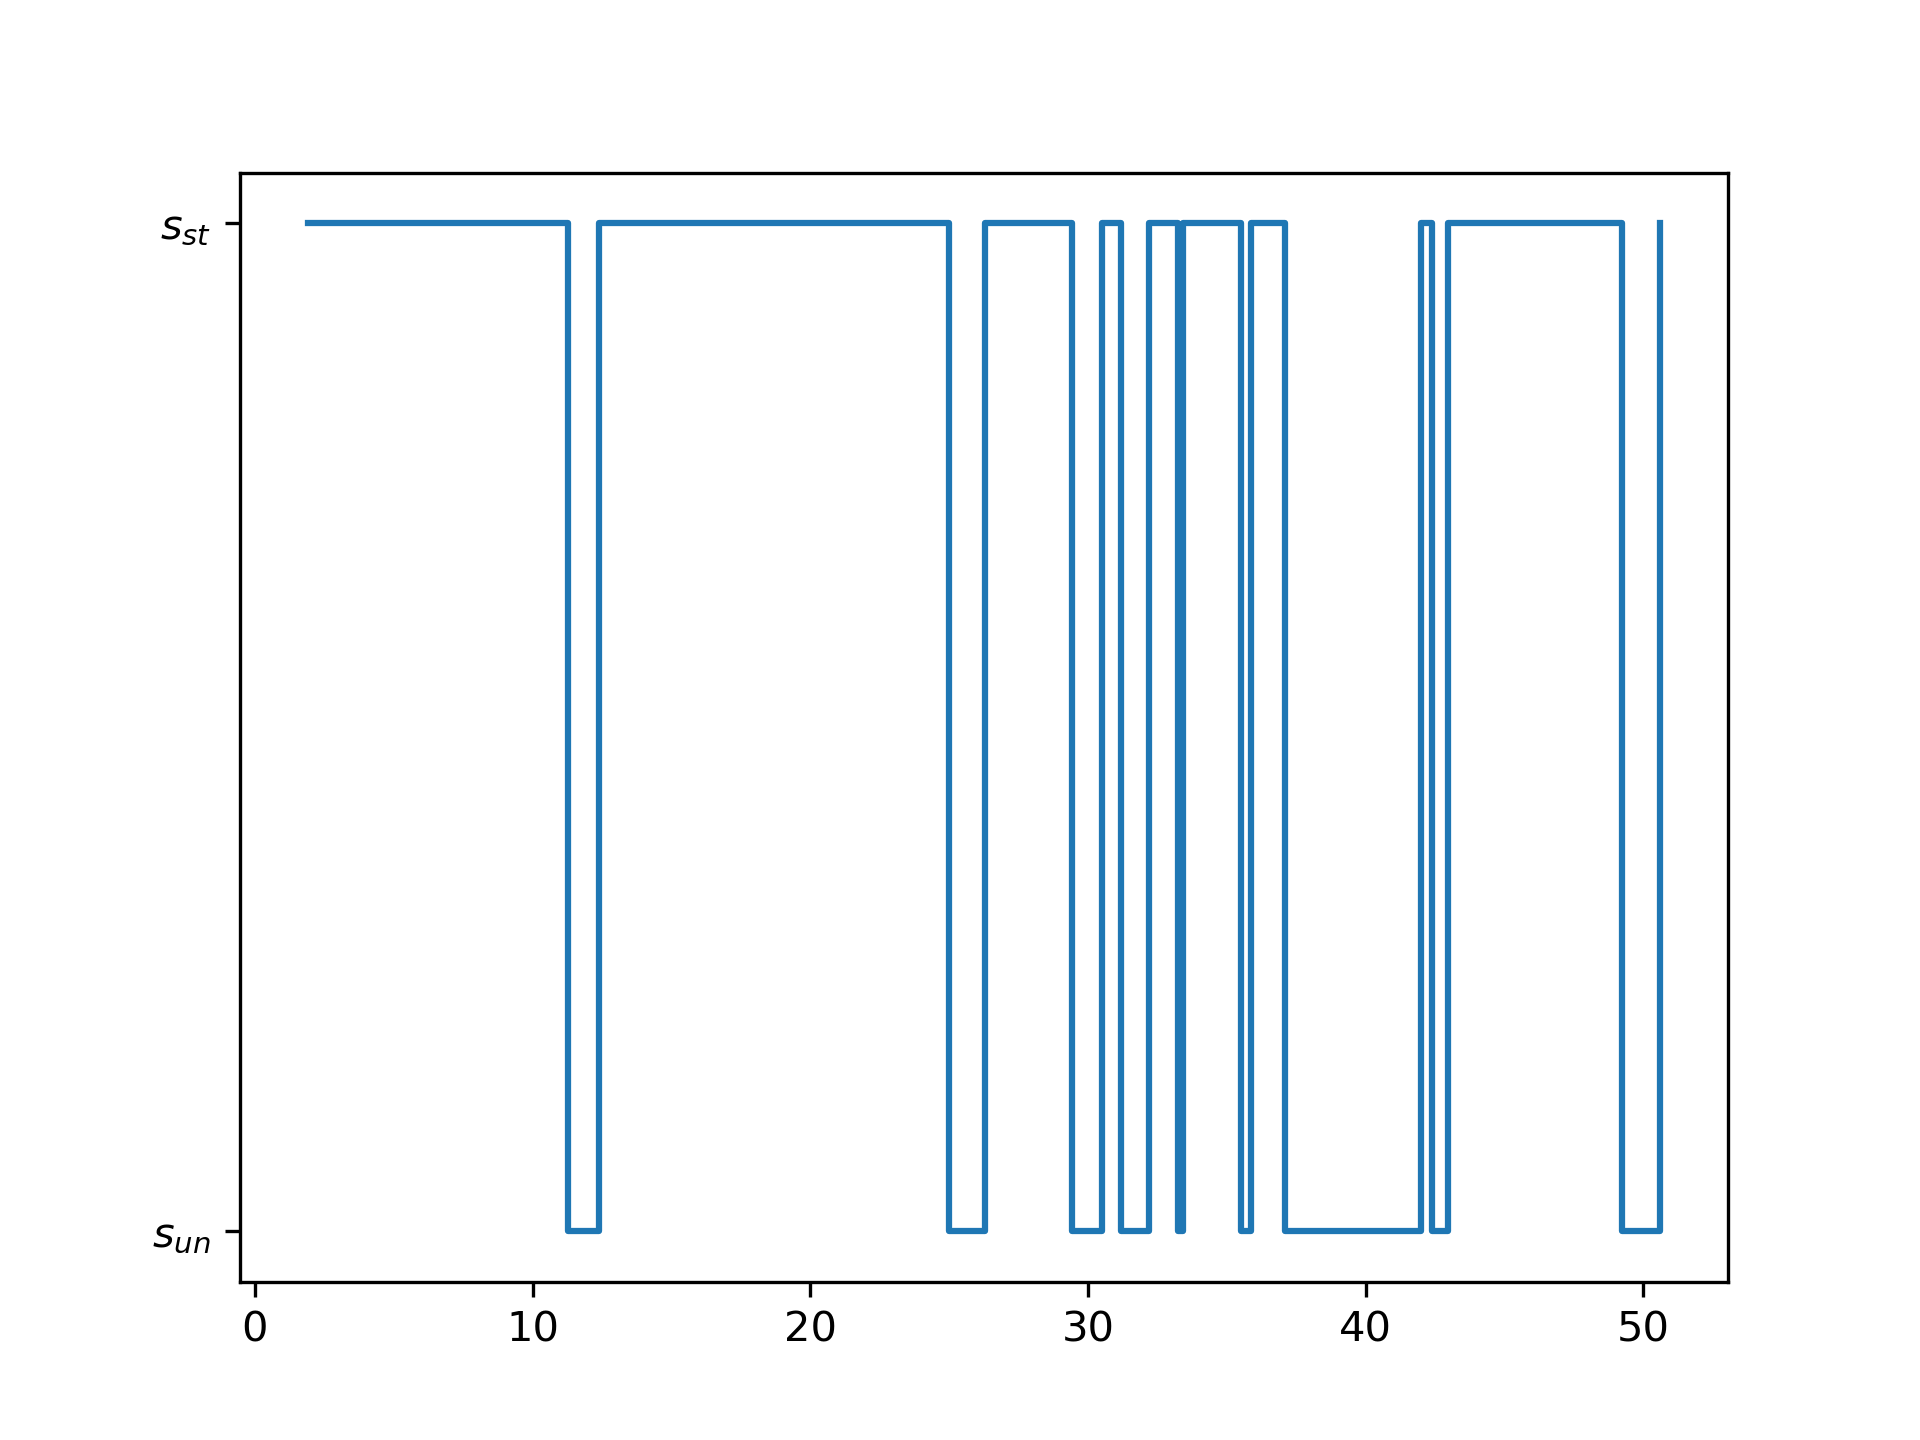
\includegraphics[width=0.75\textwidth]{../../src/2b_traj.png}
	\caption{A sample trajectory for the two-state Markov jump process with $\nu = 0.75$, $\mu = 0.25$, $s_{st} = 2$, and $s_{un} = 1$.}
	\label{fig:traj_2}
\end{figure}

It then calculates the numeric apprioxmation for $\func{P}{T_{st} \leq t}$, $\func{P}{T_{un} \leq t}$, and $\ev{X}$ and compares them to the analytic formulas given above. 

Using an RNG seed of 1 and parameters $\nu = 0.75$, $\mu = 0.25$, $s_{st} = 2$, and $s_{un} = 1$, we found the one-norm error for our numerical estimates of the PDFs to be $1.49 \times 10^{-4}$ for $\func{P}{T_{st} \leq t}$ and $2.41 \times 10^{-4}$ for $\func{P}{T_{un} \leq t}$. The numerical estimate of $\ev{X}$ is $1.2535$, whle the analytic value is $1.25$.
\end{enumerate}
